\documentclass[12pt,twoside]{report}

%\usepackage{todonotes}

%\usepackage{ifthen}
\usepackage{amssymb}
\usepackage{ulem}
\usepackage{xcolor}

% Document Configuration
%%%%%%%%%%%%%%%%%%%%%%%%%%%%%%%%%%%%%%%%%%%%%%%%%%%%%%%%%%%%%%%%%%%%%%

\usepackage{tabularx}
\usepackage{longtable}
\usepackage{ltxtable}
\usepackage{booktabs}
\usepackage{array}
\usepackage{collcell}
\usepackage{trimspaces}
\usepackage{multirow}
\usepackage{rotating}

%%%
%%% Formatting
%%%

% New rule type
\newcommand{\topruleb}{\midrule[\heavyrulewidth]}

% Commands to control the alignment of headers
\newcommand{\bfu}[1]{\textbf{\uppercase{#1}}}
\newcommand{\headingl}[1]{\multicolumn{1}{l}{\bfu{#1}}}
\newcommand{\headingc}[1]{\multicolumn{1}{c}{\bfu{#1}}}
\newcommand{\headingr}[1]{\multicolumn{1}{r}{\bfu{#1}}}

% Regular column types
\newcolumntype{x}{>{\collectcell\textsc}l<{\endcollectcell}}
\newcolumntype{y}{>{\collectcell\textsc}c<{\endcollectcell}}
\newcolumntype{z}{>{\collectcell\textsc}r<{\endcollectcell}}
\newcolumntype{u}{>{\collectcell\uppercase}l<{\endcollectcell}}
\newcolumntype{v}{>{\collectcell\uppercase}c<{\endcollectcell}}
\newcolumntype{w}{>{\collectcell\uppercase}r<{\endcollectcell}}
\newcolumntype{U}{>{\bfseries\collectcell\uppercase}l<{\endcollectcell}}
\newcolumntype{V}{>{\bfseries\collectcell\uppercase}c<{\endcollectcell}}
\newcolumntype{W}{>{\bfseries\collectcell\uppercase}r<{\endcollectcell}}

% Paragraph column types
\newcolumntype{L}{>{\raggedright\arraybackslash}X}
\newcolumntype{C}{>{\centering\arraybackslash}X}
\newcolumntype{R}{>{\raggedleft\arraybackslash}X}

\usepackage{xspace}
\usepackage{lipsum}
\usepackage{xcolor}

% Short verbatim can be formatted using \!text!: e.g., \!boolean!
\def\!#1!{\texttt{#1}}

% Acronyms should be placed in angled brackets: e.g., \<UML>
\def\<#1>{\lowercase{\textsc{#1}}}

% Abbreviations for references
\newcommand{\Figure}{Figure\@\xspace}
\newcommand{\Figures}{Figures\@\xspace}
\newcommand{\Table}{Table\@\xspace}
\newcommand{\Tables}{Tables\@\xspace}
\newcommand{\Section}{Section\@\xspace}
\newcommand{\Sections}{Sections\@\xspace}
\newcommand{\Appendix}{Appendix\@\xspace}
\newcommand{\Appendices}{Appendices\@\xspace}


% Common abbrev. are set as commands to ensure proper spacing after the dot
\newcommand{\ie}{i.e.\@\xspace}
\newcommand{\Ie}{I.e.\@\xspace}
\newcommand{\cf}{cf.\@\xspace}
\newcommand{\Cf}{Cf.\@\xspace}
\newcommand{\eg}{e.g.\@\xspace}
\newcommand{\Eg}{E.g.\@\xspace}
\newcommand{\etal}{et al.\@\xspace}
\newcommand{\etc}{etc.\@\xspace}

% Sample text
%\newcommand{\stext}[1][1-2]{\textcolor{gray!80!red}{\lipsum[#1]}}
\newcommand{\stext}[1][1-2]{\lipsum[#1]}

% Sample paragraph
\newcommand{\spar}{\stext[1]}

% Short sample paragraph
\newcommand{\sspar}{\stext[66]}
\usepackage{enumitem}
\usepackage{relsize}
\usepackage{textcomp}
\usepackage{rotating}
\usepackage{graphbox}
\usepackage{float}
\usepackage{xfrac}
\usepackage{placeins}
\usepackage{subcaption}
\usepackage[numbers,sort]{natbib}

\usepackage{acronym}
\renewcommand*{\aclabelfont}[1]{\textcolor{blue}{#1}}
%\renewcommand*{\acsfont}[1]{\textsc{#1}}

\usepackage{url}
% Allow breaking URLs at any character
\expandafter\def\expandafter\UrlBreaks\expandafter{\UrlBreaks%
  \do\a\do\b\do\c\do\d\do\e\do\f\do\g\do\h\do\i\do\j%
  \do\k\do\l\do\m\do\n\do\o\do\p\do\q\do\r\do\s\do\t%
  \do\u\do\v\do\w\do\x\do\y\do\z\do\A\do\B\do\C\do\D%
  \do\E\do\F\do\G\do\H\do\I\do\J\do\K\do\L\do\M\do\N%
  \do\O\do\P\do\Q\do\R\do\S\do\T\do\U\do\V\do\W\do\X%
  \do\Y\do\Z}

% Allow hyphenation in texttt
\LetLtxMacro\origttfamily\ttfamily
\DeclareRobustCommand*{\ttfamily}{%
  \origttfamily
  \hyphenchar\font=`\-\relax
  \fontdimen3\font=.25em\relax
  \fontdimen4\font=.167em\relax
  \fontdimen7\font=.167em\relax
}
%\definecolor{gray97}{gray}{.97}
\definecolor{gray75}{gray}{.75}
\definecolor{gray45}{gray}{.45}
\definecolor{gray20}{gray}{.20}

\definecolor{codeblue}{rgb}{0.2,0.6,.6}
\definecolor{codegreen}{rgb}{0,0.6,0}
\definecolor{codegray}{rgb}{0.5,0.5,0.5}
\definecolor{codepurple}{rgb}{0.58,0,0.82}
\definecolor{backcolour}{rgb}{0.95,0.95,0.92}



\lstdefinestyle{mystyle}{
    backgroundcolor=\color{backcolour},   
    commentstyle=\color{codegreen},
    keywordstyle=\color{black}\textbf,
    numberstyle=\tiny\color{codegray},
    stringstyle=\color{codepurple},
    basicstyle=\footnotesize,
    breakatwhitespace=false,         
    breaklines=true,                 
    captionpos=b,                    
    keepspaces=true,                 
    numbers=left,                    
    numbersep=5pt,                  
    showspaces=false,                
    showstringspaces=false,
    showtabs=false,                  
    tabsize=2,
    morekeywords={confidences,artefacts,fragments,relationshiptypes,relationshiptype,DomainType,EngineeringType,Trace,tracelinks,NodeTraceLink,LeafTraceLink,source,target,successors,referee,confidence,agents,HumanAgent,MachineAgent,Confidence,value,evidences,AIEvidence,agency,algorithmUsed,parameters,executionDate,trainingResults,impactedElements}
}
\lstdefinestyle{mystylesysml}{
    backgroundcolor=\color{backcolour},   
    commentstyle=\color{codepurple}\textit,
    morecomment=[s][\color{codegreen}]{/**}{*/},
    morecomment=[s][\color{codegreen}]{/*}{*/},
    keywordstyle=\color{codepurple}\textbf,
    numberstyle=\tiny\color{codegray},
    stringstyle=\color{codegray},
    basicstyle=\footnotesize,
    breakatwhitespace=false,         
    breaklines=true,                 
    captionpos=b,                    
    keepspaces=true,                 
    numbers=left,                    
    numbersep=5pt,                  
    showspaces=false,                
    showstringspaces=false,
    showtabs=false,                  
    tabsize=2,
    linewidth=14cm,
    xleftmargin=4.2cm,
    frame=shadowbox,
    rulesepcolor=\color{blue},
   morekeywords={confidences,artefacts,fragments,relationshiptypes,relationshiptype,Trace,tracelinks,NodeTraceLink,LeafTraceLink,source,target,successors,referee,agents,value,evidences,agency,algorithmUsed,parameters,executionDate,trainingResults,impactedElements,from,trace,class,feature,to,impacts,package,attribute,def,import,metadata,about,assert,constraint,connect,connection,to}
}


\lstdefinestyle{mystylexcore}{
    backgroundcolor=\color{backcolour},   
    commentstyle=\color{codegreen},
    keywordstyle=\color{codeblue}\textbf,
    numberstyle=\tiny\color{codegray},
    stringstyle=\color{codepurple},
    basicstyle=\footnotesize,
    breakatwhitespace=false,         
    breaklines=true,                 
    captionpos=b,                    
    keepspaces=true,                 
    numbers=left,                    
    numbersep=5pt,                  
    showspaces=false,                
    showstringspaces=false,
    showtabs=false,                  
    tabsize=2,
    morekeywords={class,contains,abstract,extends,\{,\},\[,\],refers,derived,String,get,int,double},
    linewidth=14.5cm,
    xleftmargin=2.3cm
}

\lstdefinestyle{mystyleocl}{
    backgroundcolor=\color{backcolour},   
    commentstyle=\color{codegreen},
    keywordstyle=\color{black}\textbf,
    numberstyle=\tiny\color{codegray},
    stringstyle=\color{codepurple},
    basicstyle=\ttfamily\footnotesize,
    breakatwhitespace=false,         
    breaklines=true,                 
    captionpos=b,                    
    keepspaces=true,                 
    numbers=left,                    
    numbersep=5pt,                  
    showspaces=false,                
    showstringspaces=false,
    showtabs=false,                  
    tabsize=2,
    morekeywords={context,inv,includesAll,collect,self}
}

\lstdefinestyle{mystylextext}{
    backgroundcolor=\color{backcolour},   
    commentstyle=\color{codegreen},
    keywordstyle=\color{black}\textbf,
    numberstyle=\tiny\color{codegray},
    stringstyle=\color{codepurple},
    basicstyle=\ttfamily\footnotesize,
    breakatwhitespace=false,         
    % breaklines=true,                 
    captionpos=b,                    
    keepspaces=true,                 
    numbers=left,                    
    numbersep=5pt,                  
    showspaces=false,                
    showstringspaces=false,
    showtabs=false,                  
    tabsize=2,
    morekeywords={context,inv,includesAll,collect,self},
    linewidth=14cm,
    xleftmargin=0cm
}

%\usepackage{tikz}
\usetikzlibrary{arrows}
\usetikzlibrary{shapes}
\usetikzlibrary{patterns}
\usetikzlibrary{positioning}
\usetikzlibrary{calc}
\usetikzlibrary{trees}

\newcommand*{\stereotype}[1]{
  <<{#1}>>
}

\newcommand*{\datatype}[1]{
  \stereotype{datatype}\\
  #1
}

\newcommand*{\enum}[1]{
  \stereotype{enumeration}\\
  #1
}

\newcommand*{\obj}[2]{
  \underline{{#1}~:~{#2}}
}

\newcommand*{\attributes}[1]{
  \nodepart{second}
  \begin{tabular}{@{}l@{}}
  #1
  \end{tabular}
}

\newcommand*{\literals}[1]{
  \nodepart{second}
  \ttfamily
  \begin{tabular}{@{}l@{}}
  #1
  \end{tabular}
}

\newcommand*{\operations}[1]{
  \nodepart{third}
  \begin{tabular}{@{}l@{}}
  #1
  \end{tabular}
}

\tikzstyle{reportcolor}=[
  draw=black,
  line width = 0.4pt
]

\tikzstyle{box}=[
  reportcolor,
  rectangle,
  align=center,
  minimum width=5em
]

\tikzstyle{abstractbox}=[box,
  every text node part/.style={
    font=\itshape
  }
]

\tikzstyle{class}=[box,
  rectangle split,
  rectangle split parts=2,
  minimum width=9em,
  rectangle split part align={center, left}
]

\tikzstyle{classop}=[class,
  rectangle split parts=3,
  rectangle split part align={center, left, left}
]
  
\tikzstyle{object}=[class]

\tikzstyle{abstractclass}=[class,
  every text node part/.style={
    font=\itshape
  }
]

\tikzstyle{enum}=[class]

\tikzstyle{datatype}=[class]

\tikzstyle{inherits}=[reportcolor, ->, > = open triangle 90]

\tikzstyle{contains}=[reportcolor, diamond->, > = angle 45]

\tikzstyle{assoc}=[reportcolor, ->, > = angle 45]

\tikzstyle{biassoc}=[reportcolor, <->, > = angle 45]



\usepackage{xcolor}
\usepackage{ifthen}
\usepackage{amssymb}
\usepackage{tabto}
\usepackage[page]{pagenote}
\makepagenote

\newlength\cindent
\setlength\cindent{1.5em}
\renewcommand{\notesname}{\uppercase{Notes for Clarifications}}
\renewcommand*{\notedivision}{\section*{\notesname}}
\renewcommand*{\sectionname}{\uppercase{Section}}
\renewcommand{\notenumintext}[1]{\textsuperscript{\textcolor{red}{#1}}}
\renewcommand{\thepagenote}{\roman{pagenote}}
\renewcommand{\prenoteinnotes}{\par\hangindent=\cindent\hangafter=1\noindent}
\renewcommand{\postnoteinnotes}{\par}
\renewcommand{\noteentry}[4]{%
\prenoteinnotes
\noteidinnotes{#1}{#2}%
\tabto{\cindent}%
\noteinnotes{#3}\dotfill%
\textcolor{blue}{\pageinnotes{#4}}%
\vspace{6pt}
\postnoteinnotes}

\makeatletter
\def\blankfootnote{\xdef\@thefnmark{}\@footnotetext}
\makeatother



\newcommand{\clarify}[2]{%
  {\color{red}%
      #1%
    \ifthenelse{\equal{#2}{}}{%
    }{%
      \addtocounter{pagenote}{1}%
      \blankfootnote{\color{red}\textsuperscript{\thepagenote}~#2}%
      \addtocounter{pagenote}{-1}%
    }%
  }%
  \ifthenelse{\equal{#1}{}}{%
    \ifthenelse{\equal{#2}{}}{%
    }{%
      \pagenote{#2}%
    }%
  }{%
    \ifthenelse{\equal{#2}{}}{%
      \pagenote{\textcolor{blue}{#1}}%
    }{%
      \pagenote{\textcolor{blue}{#1} --- #2}%
    }%
  }%
} 

%For code listings:
\usepackage{listings}
\usepackage{parcolumns}


\definecolor{gray97}{gray}{.97}
\definecolor{gray75}{gray}{.75}
\definecolor{gray45}{gray}{.45}
\definecolor{gray20}{gray}{.20}

\definecolor{codeblue}{rgb}{0.2,0.6,.6}
\definecolor{codegreen}{rgb}{0,0.6,0}
\definecolor{codegray}{rgb}{0.5,0.5,0.5}
\definecolor{codepurple}{rgb}{0.58,0,0.82}
\definecolor{backcolour}{rgb}{0.95,0.95,0.92}



\lstdefinestyle{mystyle}{
    backgroundcolor=\color{backcolour},   
    commentstyle=\color{codegreen},
    keywordstyle=\color{black}\textbf,
    numberstyle=\tiny\color{codegray},
    stringstyle=\color{codepurple},
    basicstyle=\footnotesize,
    breakatwhitespace=false,         
    breaklines=true,                 
    captionpos=b,                    
    keepspaces=true,                 
    numbers=left,                    
    numbersep=5pt,                  
    showspaces=false,                
    showstringspaces=false,
    showtabs=false,                  
    tabsize=2,
    morekeywords={confidences,artefacts,fragments,relationshiptypes,relationshiptype,DomainType,EngineeringType,Trace,tracelinks,NodeTraceLink,LeafTraceLink,source,target,successors,referee,confidence,agents,HumanAgent,MachineAgent,Confidence,value,evidences,AIEvidence,agency,algorithmUsed,parameters,executionDate,trainingResults,impactedElements}
}
\lstdefinestyle{mystylesysml}{
    backgroundcolor=\color{backcolour},   
    commentstyle=\color{codepurple}\textit,
    morecomment=[s][\color{codegreen}]{/**}{*/},
    morecomment=[s][\color{codegreen}]{/*}{*/},
    keywordstyle=\color{codepurple}\textbf,
    numberstyle=\tiny\color{codegray},
    stringstyle=\color{codegray},
    basicstyle=\footnotesize,
    breakatwhitespace=false,         
    breaklines=true,                 
    captionpos=b,                    
    keepspaces=true,                 
    numbers=left,                    
    numbersep=5pt,                  
    showspaces=false,                
    showstringspaces=false,
    showtabs=false,                  
    tabsize=2,
    linewidth=14cm,
    xleftmargin=4.2cm,
    frame=shadowbox,
    rulesepcolor=\color{blue},
   morekeywords={confidences,artefacts,fragments,relationshiptypes,relationshiptype,Trace,tracelinks,NodeTraceLink,LeafTraceLink,source,target,successors,referee,agents,value,evidences,agency,algorithmUsed,parameters,executionDate,trainingResults,impactedElements,from,trace,class,feature,to,impacts,package,attribute,def,import,metadata,about,assert,constraint,connect,connection,to}
}


\lstdefinestyle{mystylexcore}{
    backgroundcolor=\color{backcolour},   
    commentstyle=\color{codegreen},
    keywordstyle=\color{codeblue}\textbf,
    numberstyle=\tiny\color{codegray},
    stringstyle=\color{codepurple},
    basicstyle=\footnotesize,
    breakatwhitespace=false,         
    breaklines=true,                 
    captionpos=b,                    
    keepspaces=true,                 
    numbers=left,                    
    numbersep=5pt,                  
    showspaces=false,                
    showstringspaces=false,
    showtabs=false,                  
    tabsize=2,
    morekeywords={class,contains,abstract,extends,\{,\},\[,\],refers,derived,String,get,int,double},
    linewidth=14.5cm,
    xleftmargin=2.3cm
}

\lstdefinestyle{mystyleocl}{
    backgroundcolor=\color{backcolour},   
    commentstyle=\color{codegreen},
    keywordstyle=\color{black}\textbf,
    numberstyle=\tiny\color{codegray},
    stringstyle=\color{codepurple},
    basicstyle=\ttfamily\footnotesize,
    breakatwhitespace=false,         
    breaklines=true,                 
    captionpos=b,                    
    keepspaces=true,                 
    numbers=left,                    
    numbersep=5pt,                  
    showspaces=false,                
    showstringspaces=false,
    showtabs=false,                  
    tabsize=2,
    morekeywords={context,inv,includesAll,collect,self}
}

\lstdefinestyle{mystylextext}{
    backgroundcolor=\color{backcolour},   
    commentstyle=\color{codegreen},
    keywordstyle=\color{black}\textbf,
    numberstyle=\tiny\color{codegray},
    stringstyle=\color{codepurple},
    basicstyle=\ttfamily\footnotesize,
    breakatwhitespace=false,         
    % breaklines=true,                 
    captionpos=b,                    
    keepspaces=true,                 
    numbers=left,                    
    numbersep=5pt,                  
    showspaces=false,                
    showstringspaces=false,
    showtabs=false,                  
    tabsize=2,
    morekeywords={context,inv,includesAll,collect,self},
    linewidth=14cm,
    xleftmargin=0cm
}



% Standard shortcuts
\newcommand{\eg}{\emph{e.g.,~}}							% exempli gratia (for the sake of example)
\newcommand{\ie}{\emph{i.e.,~}}							% id est (that is)
\newcommand{\Fig}[1]{Fig.~\ref{#1}}  			% choose Fig. or Figure, depending on the style
\newcommand{\Table}[1]{Table~\ref{#1}}	    % Table reference
\newcommand{\Sect}[1]{Section~\ref{#1}}	  % section name always with a capital S
\newcommand{\Model}[1]{\textsf{\small{#1}}} % name of any modeling artifact (e.g., formalism, model element, rule, ...)
\newcommand{\Code}[1]{\texttt{\small{#1}}}	% inline code
\providecommand{\e}[1]{\ensuremath{\times 10^{#1}}}	% scientific notation: x.10^y

%%%%%%%%%%%%%%%%%%%%%%%%%%%%%%%%%%%%%%%%%%%%%

% Shortcuts
\newcommand{\MOF}{\textsc{MOF}\xspace}
\newcommand{\ocl}{\textsc{OCL}\xspace}
\newcommand{\OCL}{\textsc{OCL}\xspace}
\newcommand{\nsga}{\textsc{NSGA-II}\xspace}
\newcommand{\MDE}{\textsc{MDE}\xspace}
\newcommand{\MT}{\textsc{MT}\xspace}
\newcommand{\WFR}{\textsc{WFR}\xspace}
\newcommand{\Ecore}{\textsc{Ecore}\xspace}
\newcommand{\OURNAME}{{our approach}\xspace}



\newcommand{\ra}{$\rightarrow$}
\newcommand{\la}{$\leftarrow$}
\newcommand{\ugh}[1]{\textcolor{red}{\uwave{#1}}} % please rephrase
\newcommand{\ins}[1]{\textcolor{blue}{\uline{#1}}} % please insert
\newcommand{\del}[1]{\textcolor{red}{\sout{#1}}} % please delete
\newcommand{\chg}[2]{\textcolor{red}{\sout{#1}}{\ra}\textcolor{blue}{\uline{#2}}} % please change
\newcommand{\move}[2]{\textcolor{blue}{\uwave{#1} (Move to #2)}} % please move


\newboolean{showcomments}
\setboolean{showcomments}{true} % toggle to show or hide comments
\ifthenelse{\boolean{showcomments}}
{\newcommand{\nb}[2]{
		\fcolorbox{gray}{yellow}{\bfseries\sffamily\scriptsize#1}
		{$\blacktriangleright$#2$\blacktriangleleft$}
	}
	\newcommand{\version}{\emph{\scriptsize$-$working$-$}}
}
{\newcommand{\nb}[2]{}
	\newcommand{\version}{}
}



\newcommand\eb[1]{\nb{EB}{\textcolor{red}{\textsl{#1}}}}
\newcommand\jc[1]{\nb{JC}{\textcolor{red}{\textsl{#1}}}}
\newcommand{\todo}[1]{\textbf{\textcolor{red}{TODO: #1}}}
\newcommand\syn[0]{\fcolorbox{gray}{green}{\bfseries\sffamily\scriptsize{SYN.}}}

\newcommand\bluefat[1]{$\blacktriangleright$\textcolor{blue}{\textit{#1}}$\blacktriangleleft$}
\newcommand\blue[1]{\textcolor{blue}{#1}}
\newcommand\red[1]{\textcolor{red}{#1}}

\makeatletter
\def\ughu{\bgroup \markoverwith{\lower3.5\p@\hbox{\sixly \textcolor{red}{\char58}}}\ULon}
\font\sixly=lasy6 % does not re-load if already loaded, so no memory problem.
\makeatother


\newcommand\missref[1]{\ughu{#1}~\ugh{[?]}}

% Document Configuration 
%%%%%%%%%%%%%%%%%%%%%%%%%%%%%%%%%%%%%%%%%%%%%%%%%%%%%%%%%%%%%%%%%%%%%%
 
% \title{3\textsuperscript{rd} Deliverable:\\Traceability Solutions \\ -- Evaluation and extension ~~~~~~~~~~ -- APPLICATION TO capra}
\title{3\textsuperscript{rd} Deliverable:\\Traceability solutions \\ -- Evaluation and extension}

\author{
  Edouard R. Batot 
} 

\date{ 
  April 23, 2021
}

% Begin document
%%%%%%%%%%%%%%%%%%%%%%%%%%%%%%%%%%%%%%%%%%%%%%%%%%%%%%%%%%%%%%%%%%%%%%

\begin{document}

% Title page
\maketitle 

\title{3\textsuperscript{rd} Deliverable:\\Traceability Solutions -- Evaluation and extension}

% Table of Contents
\tableofcontents

% Contents
\cleardoublepage
\renewcommand{\sectionbreak}{}
%!TEX root = ../document.tex
\section*{List of Acronyms}
\begin{descriptioncompact}
    \item[MDE] {Model-Driven Engineering}
    \item[MBSE] {Model-Based Sofware Engineering}
    \item[DSML] {Domain Specific Modelling Language}
    % \item[UML] {Unified Modeling Language}
    \item[XMI] {XML Metadata Interchange}
    \item
    \item[SOM] {Systems, Software and Models Lab}
    \item[UOC] {Fundacio per a la Universitat Oberta de Catalunya}
    \item[CEA] {Commissariat à l'énergie atomique et aux énergie alternatives}
\end{descriptioncompact}

\listoffigures
\lstlistoflistings
\renewcommand{\sectionbreak}{\cleardoublepage}
\cleardoublepage


%\section*{Foreword}
%\begin{figure}[ht] 
%	
%	\centering
%	
\includegraphics[width=.7\linewidth]{images/citation-ermine.pdf}
%\end{figure}



\section{Introduction}\label{sect:intro}
This document presents the integration of Trace\textit{a} \cite{batot2021-not-another-metamodel}, a language dedicated to traceability into the new release of SysML language.
It is the continuation of deliverables 1, 2, and 3 of the Trace\textit{a} project\footnote{Trace\textit{a} is part of the Modelia intiative which aims at "Bringing artificial intelligence to the modeling world"\\ \url{https://modelia.eu/projects/}.}. The first deliverable introduces the conceptualization work (SoA) related to traceability (D1)~\cite{deliverable1}. The second presents the metamodel of a language dedicated to traceability (D2) that fills the gaps detected in the existing literature during D1~\cite{deliverable2}. The third deliverable shows the evaluation and integration of functionalities (confidence and evidence) in a software dedicated to traceability (D3)~\cite{deliverable3}.
This report presents the integration of the concepts related to traceability developed during these first three deliverables within SysMLv2\footnote{We alternately use the names SysML and SysMLv2 to refer to SysMLv2. The distinction between the two as well as all documentation relating to KerML / SysMLv2 is available by following the link:\\ \url{https://github.com/Systems-Modeling}.}.

This document is organized as follows.
\Sect{sec:background}, first briefly introduces the language dedicated to traceability that we have developed as well as the KerML / SysMLv2 ecosystem on which we integrate it. This section also defines the high level needs for quality traceability.
\Sect{sec:strategies}, presents which elements of KerML / SysMLv2 languages are of interest and how we have adapted and used them through the different integration strategies considered.
We will detail our choices of architecture and implementation and the limits that we encountered in \Sect{sec:extension}\footnote{We are integrating Trace\textit{a} into SysMLv2 while it is being formalized by the SST.}.
Finally, we conclude this document in \Sect{sec:conclusion} before pointing at the resulting software artefacts and their examples of use in \Sect{sec:artefacts}.






% \begin{descriptioncompact}
%      \item[Suite de Tracea] Livrables, objectifs
     
%      \item[Besoins de SysML] Intérêt à intégré Tracea au nouveau standard 
%      - Limitations
%      - Niveau de priorité faible (retard de livraison)
     
%      \item[Stratégies explorées] Elements du noyau (cibles de la traçabilité)
%      \begin{itemize}
%          \item  \textbf{Approches naïves/intrusives:} Modifier les éléments du noyau - Nouveau type d'annotation)
%          \item \textbf{Approches orthogonales:} Nouvelle fonction annotatrice - Bibliothèque de fonctionnalités) 
%      \end{itemize}
% \end{descriptioncompact}



\section{Evaluation protocol for traceability solutions}\label{sec:evaluation}
\sideboxbegin{o}
This section presents {a protocol to evaluate tracers}. The main focus in the consideration of the trace artefacts themselves, their customization, identification, visualization, persistence and quality assessment. It also sketches {a protocol to integrate Trace\textit{a}'s quality definition into tracers}.
\sideboxend

The quality of traceability solutions lies on five main pillars : 
(1) The customization of the tool to adapt to different systems\footnote{We call \textit{system} or \textit{software system} interchangeably here, considering a software system an abstract representation of a (software) system.}, 
(2) the level of automation of the identification of traces, 
(3) the means of visualisation and retrieval of trace links, 
(4) the means of persistence and additional operations available, 
and (5) level of quality assessment of the tracing constituents.
In this section, we present these as five independent dimensions for the evaluation of traceability solutions. 

\Fig{fig:evaluationpoints} schematizes the overall traceability infrastructure. It shows the three main components: the traces and their constituents, the environment in which it operates, and the artefacts it targets on (a) system (of systems). The figure shows where the dimensions for evaluation apply.
 
\begin{figure}[h]  
	\centering
	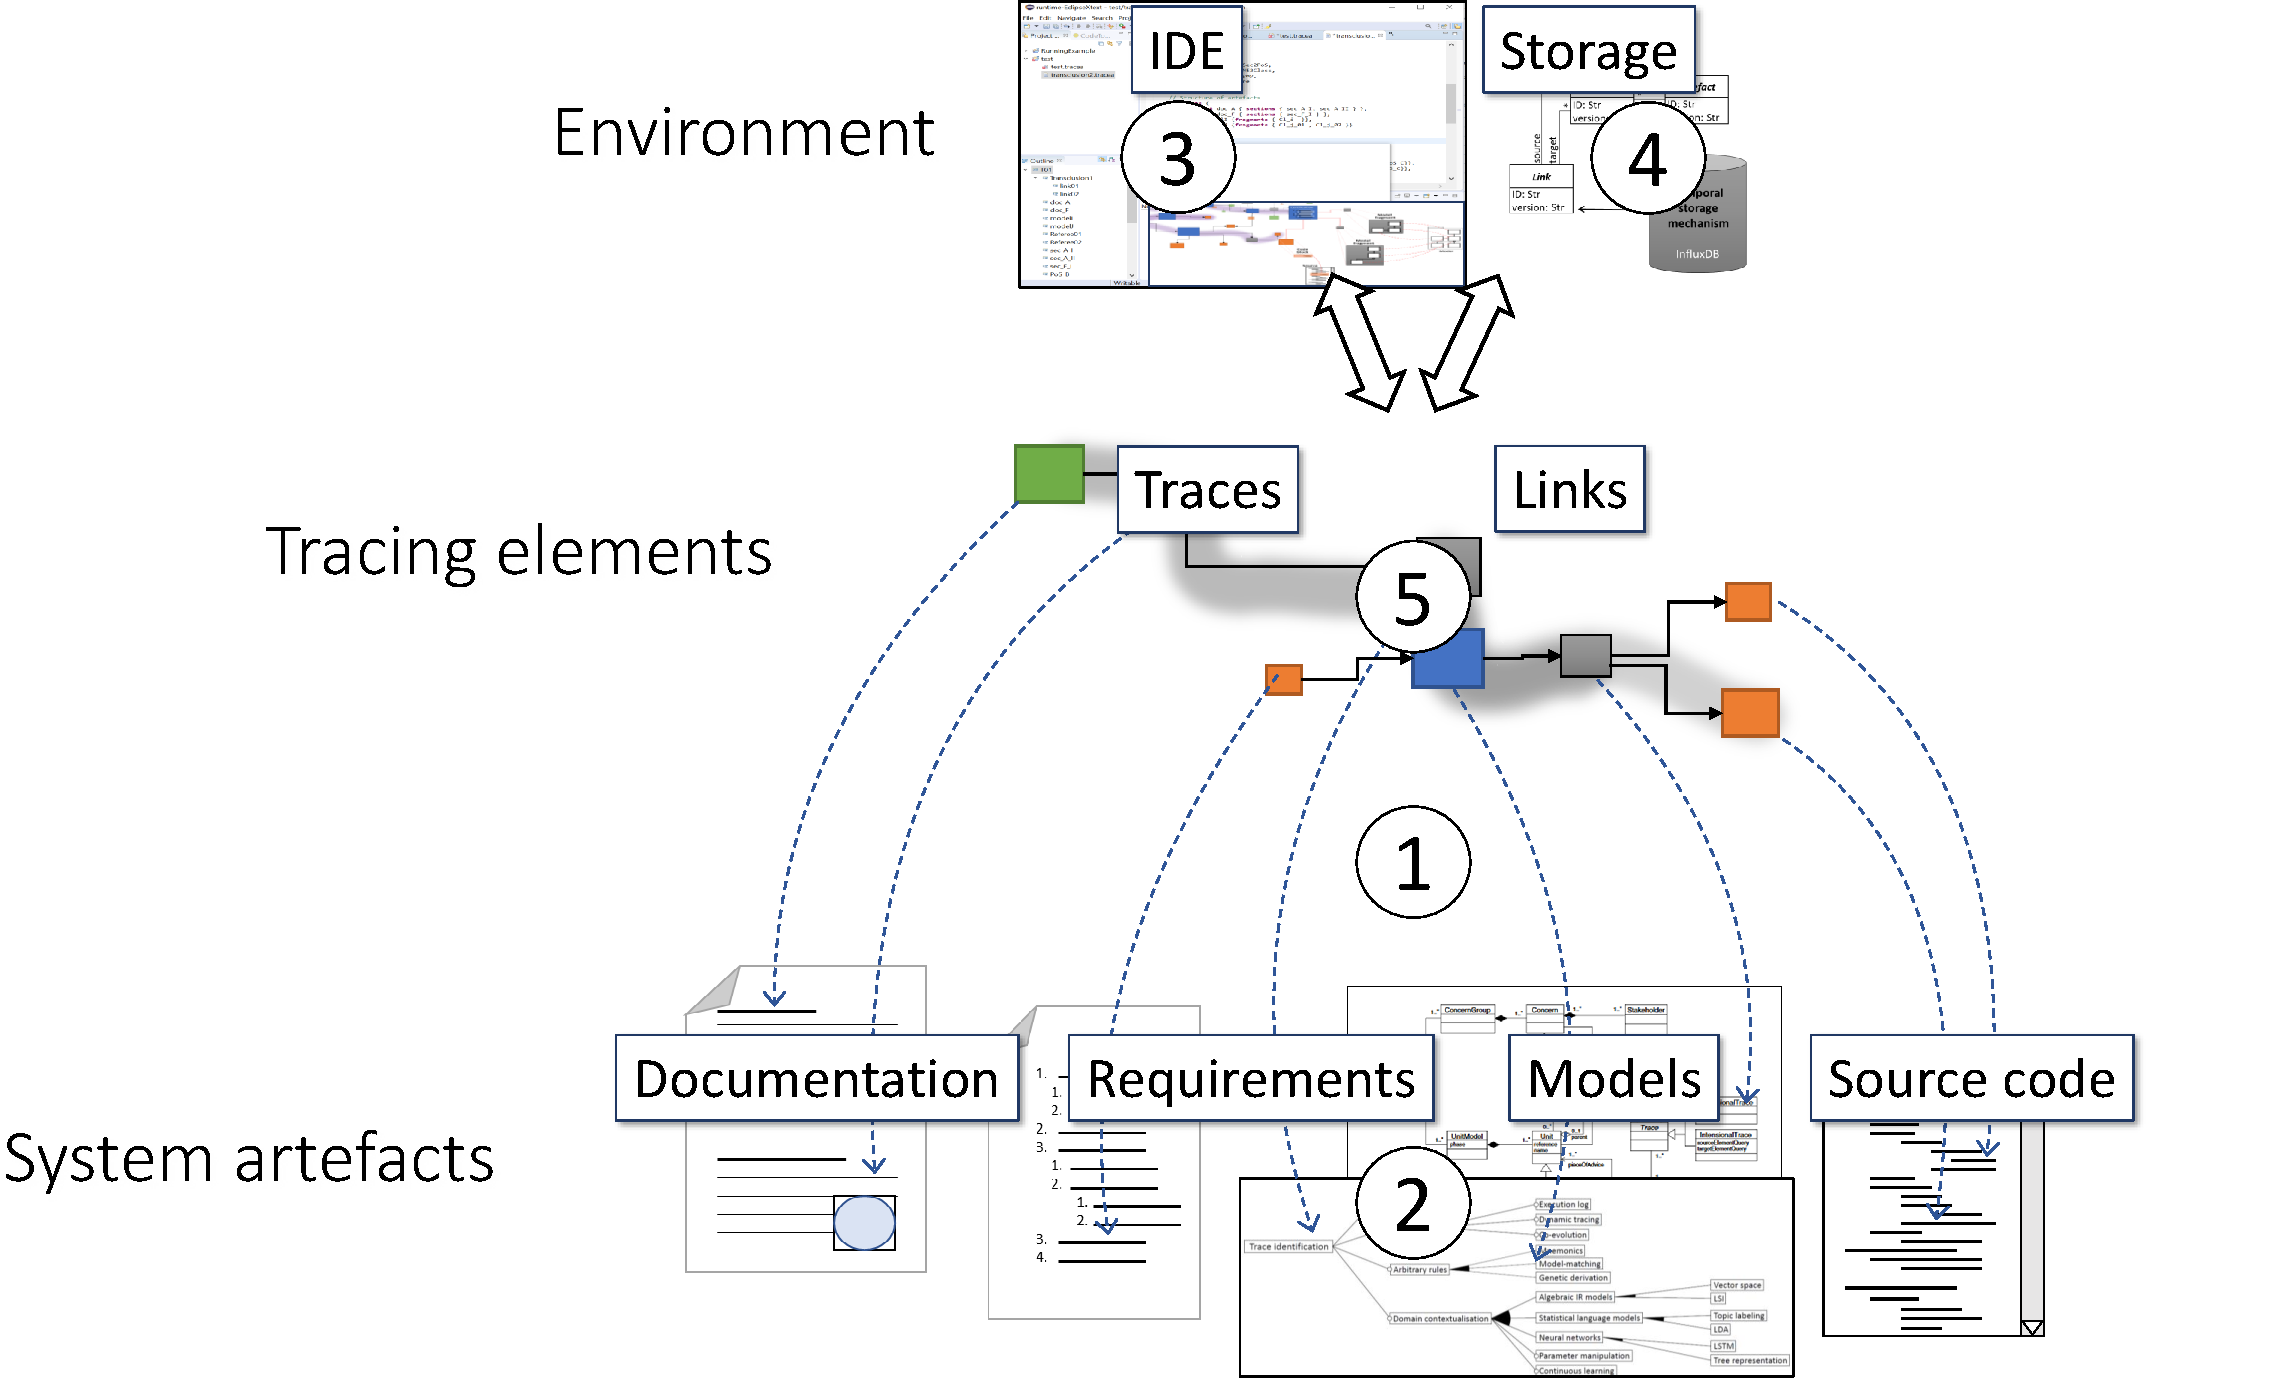
\includegraphics[width=.85\linewidth]{images/evaluation-points.pdf}
	\caption{Overview of the traceability infrastructure with localisation of the dimensions for evaluation}
	\label{fig:evaluationpoints}
\end{figure}

\subsection{Evaluation of traceability solutions}\label{sec:protocol-evaluation}
In more details, we define five dimensions to evaluate a solution to traceability (as summarized in Table \ref{tab:evaluationtable}).
\begin{table}[h]  
	\centering
	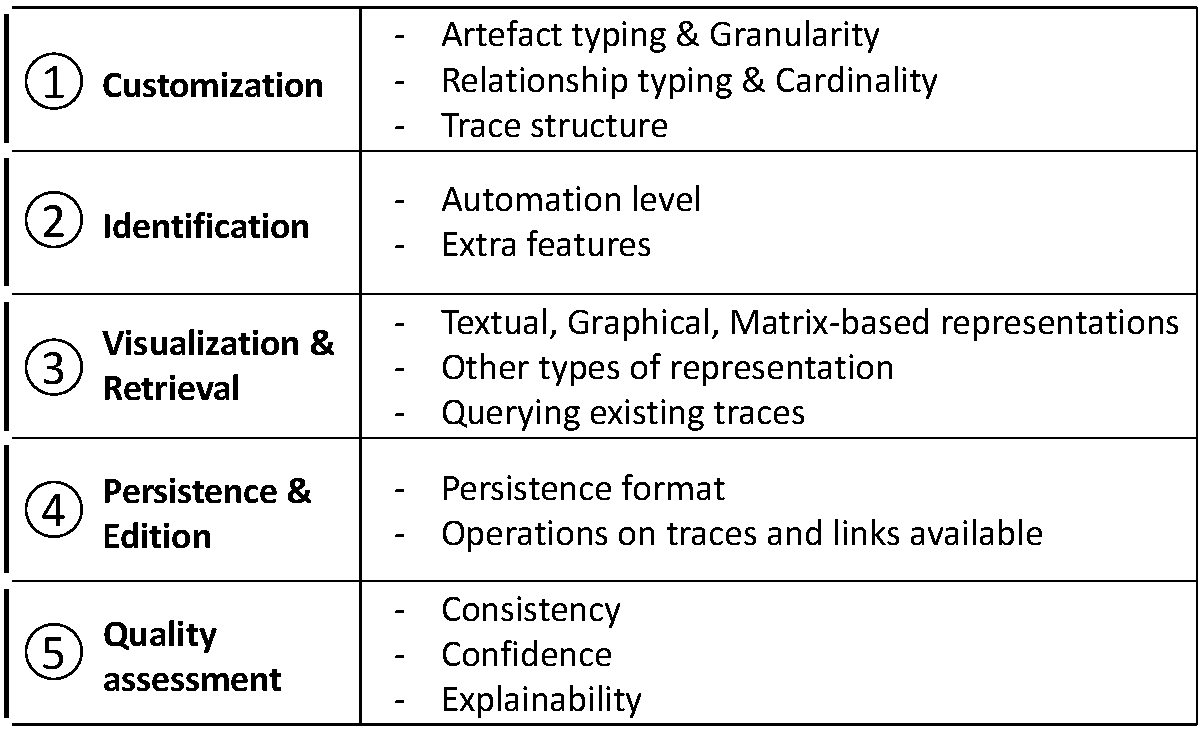
\includegraphics[width=.65\linewidth]{images/evaluation-table.pdf}
	\caption{Five pillars for traceability evaluation.}
	\label{tab:evaluationtable}
\end{table}

\begin{descriptioncompact}
    \item[1 - Customization] To evaluate the potential a tool has to address a specific purpose, \textbf{customizability} must be evaluated with regard to the kind of artefacts and the kind of links it offers to manipulate\footnote{We call "trace links", "connections", "relationships", simply \textit{links} in this document, as opposed to \textit{trace} which are entities composed with (successive) links.}. A generic tooling must allow an \textit{ad hoc} definition of types to adapt to different uses in different application domains \cite{maro2016_maintenance_factors_and_guidelines}. 
    
    \item[2 - Identification] What are the means available for the identification of trace links? This task can be automated to different levels. Links can be identified manually, which usually depends on the integration of the tool into the system's environment. Links can also be identified automatically using rules and/or AI techniques.
    Moreover, there exists explicit links in the syntax trees of many languages. These can be automatically derived, included or used for visualization purpose as an extra feature (or known neighborhood). 

    \item[3 - Visualization \& Retrieval] Once traces are identified, they can be represented in form that fit the needs of the user. \textit{E.g.}, either textually, or diagramatically, in spreadsheet or even in matrix, revealing their structure in a (more or less) legible way, and editable to a certain degree.  
    Matrix-based representations show a broader aspect of the traces in a more "conventional" way that some favor \cite{li2013-trace-matrix-analyzer}. For example, the matrix view makes it easy to see if all requirements are associated to test cases.
    
    There might as well be a great number of traces identified, for various purposes, and a proper tooling to retrieve traces of interest is important. This can be done, for example, with a query-based mechanism.

    \item[4 - Persistence \& Edition] The format in which traces are serialized matters. It can be embedded in the artefacts themselves, or external to the software through independent traceability artefacts. These can be store as model elements, SQL scripts, or XML sheets, and so on depending on traceability requirements (\textit{\eg,} what is most important: expressiveness, efficiency, or interoperability?).
    
    Traces are complex entities and a robust tooling should also offer robust operations to handle them with precision and efficacy.
    
    \item[5 - Quality assessment] Finally, how is the quality of the trace and its constituent assessed? Traces suffer gradual decay, depending on the degree of versatility of the system, they might not be kept up-to-date, and their consistency with the system's artefacts may decline. This indicates that traces might suffer some uncertainty. Is the confidence about the degree of existence of a trace evaluated? Is it possible to record and reuse it? If a trace has been identified automatically, traces should refer to evidences about the rationale behind their identification. Is the tool offering any means to express these considerations?
\end{descriptioncompact}
 

\subsection{Extension for trace quality}\label{sec:protocol-extension}
We foresee a recurring lack in the fulfilment of the last dimension "5 - Quality assessment". All approaches we have seen so far are oblivious of this aspect~\cite{deliverable2,batot2020-survey-driven-feature-model}. We propose to address this limitation through an extension protocol that integrates trace quality into traceability solutions. \Fig{fig:mm-explainability} shows an excerpt of Trace\textit{a} dedicated to the quality of traces and links. This excerpt features confidence values associated with evidences - when they exist. The root element for tracer must also refine \texttt{TracingElement} to advocate for \texttt{Agent} responsibility in the tracing process. A detailed review of {the conceptual modeling beyond trace quality classes} imported by Trace\textit{a} is provided in \cite{batot2021-not-another-metamodel}.

\begin{figure}[h]     
	\centering
	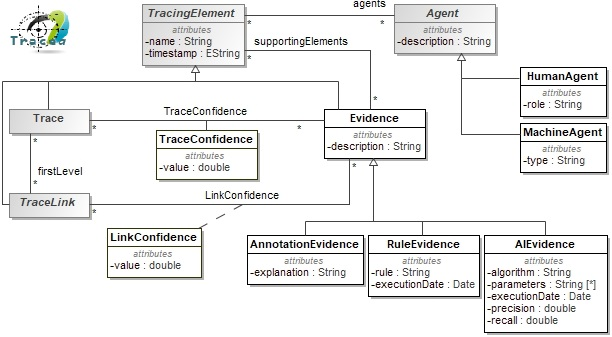
\includegraphics[width=.99\linewidth]{images/mm-explainability.jpg}
	\caption{Excerpt of Trace\textit{a} dedicated to the quality of traces and links.}
	\label{fig:mm-explainability}
\end{figure}


\begin{descriptioncompact}
    \item[1 - Localisation] First of all, we need to locate the core conceptual representation of trace link. Is it a model that generates some low level code? Is it rendered directly in low level code such as Java or C? Is it explicitly modularised or is it part of a bigger picture?
    
    
    The extension point for tracers to integrate Trace\textit{a} lies in the left-hand classes \texttt{Trace} and \texttt{TraceLink} of Fig. \ref{fig:mm-explainability}. Both are susceptible to give a confidence value, supported by evidences if any. 
    %The actual representation of traces and links must be studied as well. Are \textit{traces} actual entities? Or are they \textit{derived} from \textit{links}? 
    
    
    \item[2 - Injection] Then, Trace\textit{a} quality properties must be added to the definition. This may be done through a modification of the metamodel (in the case of low code generation) or a direct edition of low level code related to links and traces. In both cases, Trace\textit{a} must endorse a translation into the language/technology of the targeted tracer.
    
    
    
    \item[3 - Interfacing] Once quality properties have been added to the tracer, it must be propagated through the different packages/modules of the tool. This implies understanding the general architecture of the tracer to be able to add quality properties as a core feature without \textit{breaking stuff}\footnote{Facebook's mantra for developers has long been "Move Fast and Break Things." After decade long polemic over its legal implication, the Menlo Park company has stepped down. Facebook is now embracing the motto "Move Fast With Stable Infra." }.
    
    \item[4 - Change impact] Finally, a change impact analysis must be operated to ensure the changes do not impact unexpected elements of the tracer. This must be done at the specification, design, source code, and test level.
\end{descriptioncompact}




\section{Evaluation of a traceability solution: Capra}\label{sec:evaluationcapra}
\sideboxbegin{o}
This section depicts how the protocol from Section \ref{sec:protocol-evaluation} has been applied to evaluate Capra. The adaptativeness of the tool through customization and visualization features is put forward ; identification and quality assessment remain slightly back.
\sideboxend



Capra is a promising generic solution to model-based software traceability \cite{heisig2019-generic-traceability-metamodel-end-to-end-capra,maro2016_maintenance_factors_and_guidelines}. Yet, as we will see, it suffers an obvious lack of means to consider the quality of traces.
In this section, after a brief introduction to Capra, we detail the application of the protocol introduced in Section \ref{sec:protocol-evaluation} on that specific solution. We detail each of the five steps and summarize the results in Table \ref{tab:evaluationcapra} to establish whether, or to what cost, Capra would fit a consequent industrial exploitation.

\begin{descriptioncompact}
    \item[Quick presentation of Capra] Capra is a tool and a research project aiming at generic software traceability \cite{heisig2019-generic-traceability-metamodel-end-to-end-capra,maro2016_maintenance_factors_and_guidelines}. Its initiators rose the ability to trace as a noticeably important feature to integrate into the realm of model-driven engineering \cite{hotlmann2020-MB-traceability-terminology}. Scientific publications show that strong traceability has been long due in the field and Capra's authors distinguish themselves from other approaches with an important focus on customizability and visualization of tracing artefacts \cite{clelandhuang2007bestPracticeForAutomatedTraceability,mader2010-visual-tracability-modeling-language}. The overall goal of Capra is to allow the linking of elements from different domain specific modeling languages.

    \begin{figure}[h]  
    	\centering
    	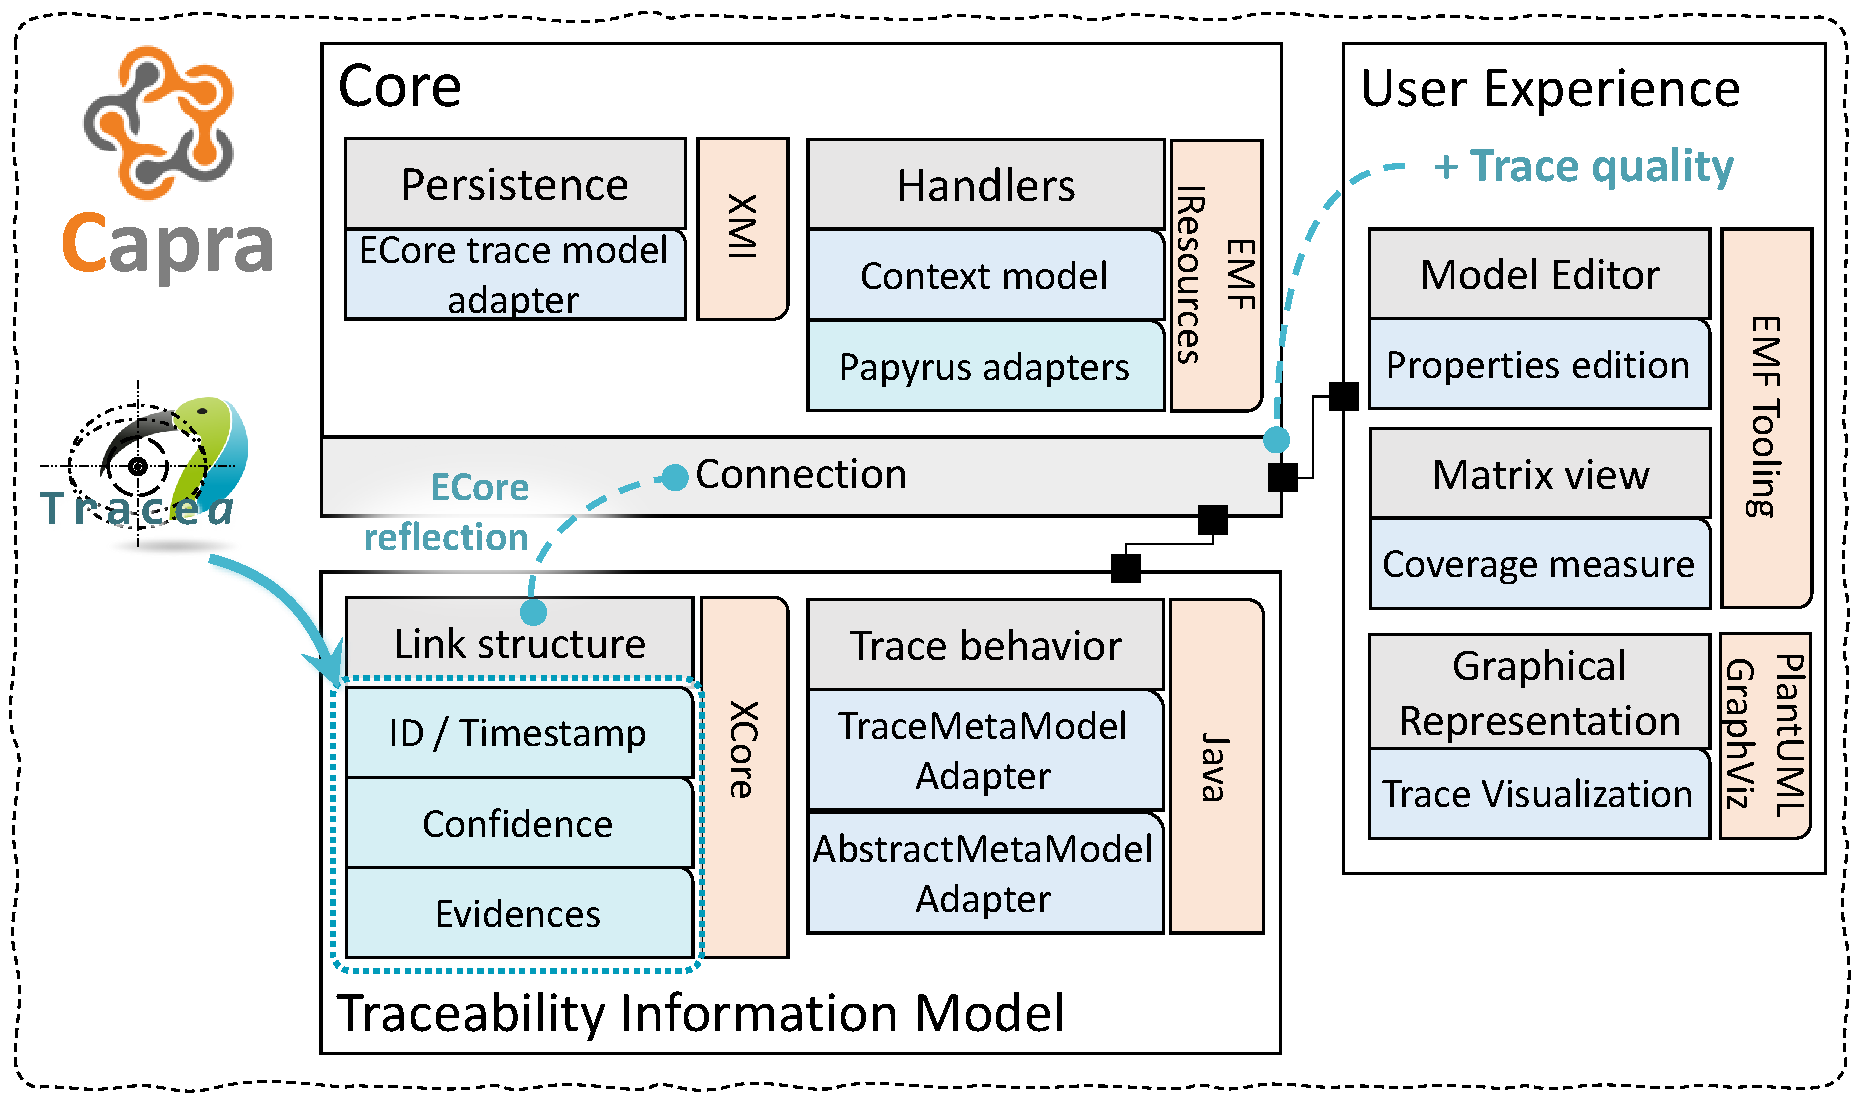
\includegraphics[width=.85\linewidth]{images/capra-architecture}
    	\caption{Architecture of Capra}
    	\label{fig:capraarchitecture}
    \end{figure}
    
    See \Fig{fig:capraarchitecture} for a detailed view of Capra architecture. The implementation of the tracer is based on the Eclipse Modeling Framework \cite{EMF} hosted open on Git \cite{Capra_Repo}. It consists of an Eclipse plugin that carries out the requirements an industrial partner mandates.  There is a core package, which grows into new handlers to support more and more domain specific languages and usages\footnote{To quote but one example, Capra is ready to use with Papyrus models and elements.}. A package is dedicated to the customization of the traceability information model (or trace model), and the UI is based on Eclipse's ECore model editor and PlantUML for diagrammatic representations.
     
    The maintenance of the tool is ensured mainly by the authors of the publications. They are quick to answer questions and comments.
    
    

\end{descriptioncompact}


\subsection{Traceability customization}\label{sec:custom}

Capra allows a custom definition of the artefacts' and relationships' types. The customization of artefacts and links is editable through an XCore plugin\footnote{More details can be found at: \url{https://wiki.eclipse.org/Capra/CustomTraceabilityMetaModel}}. Links can be defined following a hierarchical inheritance and allowing structural features (reference and attributes)\footnote{There is no guaranty on the level of implementation of the more complex features XCore allows.}. 

Capra is an EMF plugin and benefits from the artefacts used by the running instance of the platform. An artefact is defined through the resource change management plugin mechanism of EMF infrastructure. The wrapping of the artefacts uses another XCore plugin. It allows the definition of other attributes for artefacts: \verb|org.eclipse.capra.generic.artefactmodel|.
The adapters, handlers, and helpers for the EMF artefacts must be redefined as Java polymorphic overriding projects (derived from \verb|org.eclipse.capra.generic.core|).  
Capra redefines wrappers for 15 languages or standards such as UML, BPMN, Papyrus, Mylyn, Java, C++ Office, to name a few\footnote{There is no documentation relating the means to apply such redefinition - neither can be found any tips on the potential impact such changes may initiate.}. 

By default there is one generic \textit{RelatedTo} possible kind of link. For each link, there must be one and only one source and one or more target artefacts (target cardinality can be changed). The types of origin and target artefacts can be constrained.

In the default implementation, links are part of a \texttt{TraceModel} that \textit{connects} between them. There is no explicit trace structure but a \textit{behavior} defined in Java. 
If an artefact is part of the target of a link and the origin of another, the trace connects (see the Section \ref{sec:visualization} on visualization). This implementation (\verb|org.eclipse.capra.generic.GenericTraceModel|) must be transferred or adapted (Java file, no documentation) to be adapted to a new structure. There is no test coverage for potential alterations to the original implementation. 

\subsection{Links identification}\label{sec:identification}
Identifying links in Capra is done manually. Any element actionable in an Eclipse environment can be selected to take part of a trace. A context menu reacts to elements and offers to add to the "Traceability selection", or drag-n-drop the element into the \texttt{Trace Creation}\footnote{Names are subject to change.} view (\Fig{fig:tracecreation}). (Respective adapters are required, see Section \ref{sec:custom}.)
There is no automation for the identification of relationships, but the UML dependencies can be viewed in the \texttt{Capra PlantUML Viewer}. UML relations are not part of the serialized of the trace links. They are derived for (visual) convenience and they need to be manually recorded to be serialized.

\begin{figure}[h] 
	\centering
	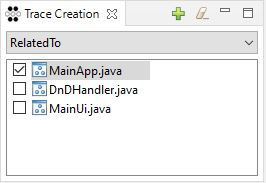
\includegraphics[width=.35\linewidth]{images/tracecreationview.JPG}
	\caption{Capra's Trace Creation view}
	\label{fig:tracecreation}
\end{figure}

\subsection{Trace visualization \& Retrieval}\label{sec:visualization}
Capra's prime feature is a multi-paradigm visualization support with textual, graphical and matrix representations. 
The second, based on PlantUML/Graphviz, supports developers in change impact analysis ; the matrix representation facilitates the evaluation of test coverage. Mixing the two allows an in depth safety analysis - Capra's authors next publication will show this last point\footnote{From an interview with the main Git contributor and author.}. 
	
\begin{descriptioncompact}
    \item[Augmented text representation of links] 
Traces in Capra are serialized into XMI Ecore models. This is convenient since Eclipse offers a \texttt{Reflexive Ecore Model Editor} to browse and edit such resources. Traces themselves cannot be apprehended though, if not to a great cost, because this view does not show the succession of trace links. \Fig{fig:xmieditor} shows a screenshot of this view. As can be seen, a name composed with the name of the artefacts targeted is the only information available - together with the elements properties in the \texttt{Properties} view associated. 
Instances of the wrappers for the artefacts used by the trace links are stored in the same manner in another XMI file.
\begin{figure}[h] 
	\centering
	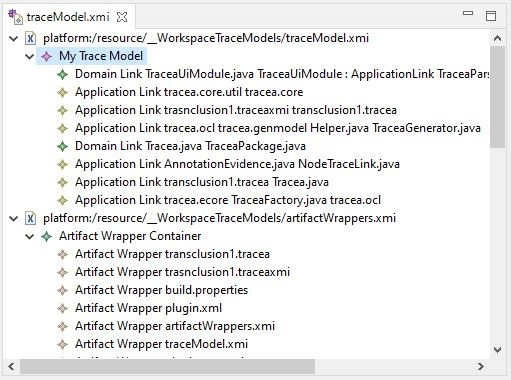
\includegraphics[width=.65\linewidth]{images/XMIEditor.jpg}
	\caption{Links and artefact wrappers, browsed with Eclipse Ecore Model editor}
	\label{fig:xmieditor}
\end{figure}

    \item[Graphical representation of traces] %using PlantUML/GraphViz plugin
To ease the visualization, Capra generates a graphical description of traces in GraphViz\footnote{\url{https://graphviz.org/}} and uses PlantUML\footnote{\url{https://plantuml.com/}} to plot them in an Eclipse view. Figure \ref{fig:plantuml} shows a capture of the view.
This view shows the links associated to the element selected in the Eclipse IDE. These links are the one {identified} with Capra (the trace links) or are derived from the neighborhood of the element selected. In the case of a Java class, a type hierarchy is provided.
The view is configurable. The type of links, as well as {the depth of transitivity} can be changed through the Eclipse interface.  
\begin{figure}[h] 
	\centering
	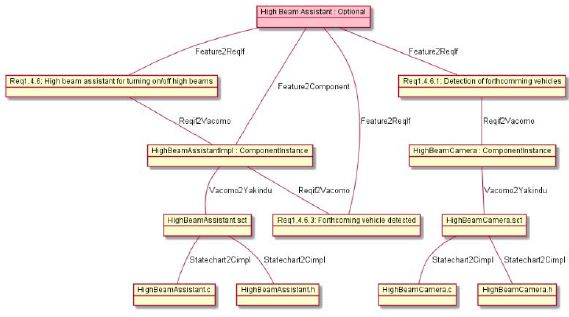
\includegraphics[width=.60\linewidth]{images/plantuml-viewer.jpg}
	\caption{Trace links sequences are plotted graphically in Capra PlantUML Viewer}
	\label{fig:plantuml}
\end{figure}

    \item[Matrix-based representation of tracing] 
%Numerous authors in traceability shows the importance of a \ughu{broader} point of view on the tracing process that shows the linkage between the traced artefacts through an association matrix. 
Capra offers an association matrix view, as can be seen in \Fig{fig:matrixviewer}. This view shows links from a high-level perspective and is most useful for coverage measurement. It can be exported in the Excel (xls) format.
\begin{figure}[h] 
	\centering
	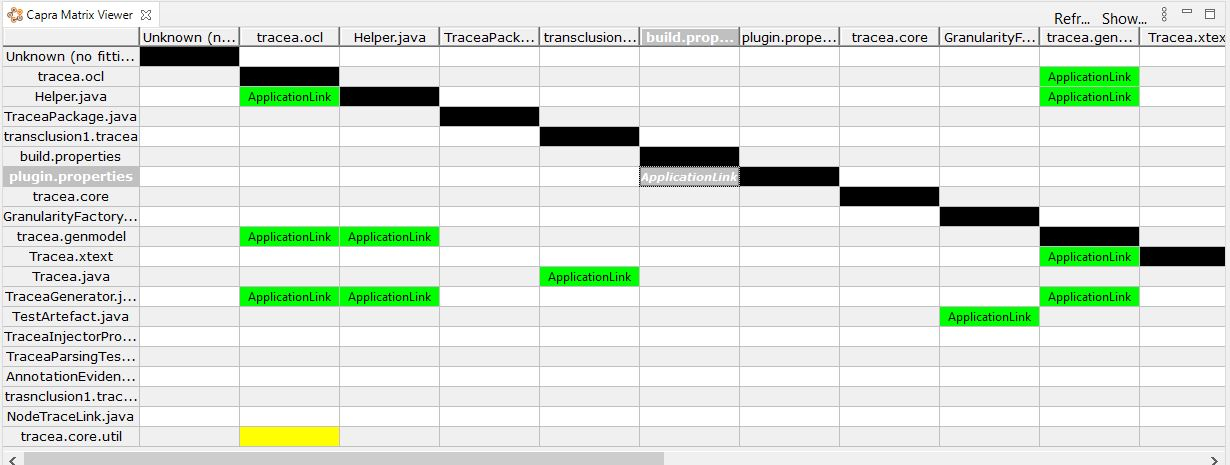
\includegraphics[width=.65\linewidth]{images/matrixViewer.jpg}
	\caption{Interrelations can be viewed in the matrix-based representation}
	\label{fig:matrixviewer}
\end{figure}

    \item[Link retrieval] There is no mechanism to retrieve automatically trace links. Yet, the use of Viatra-IncQuery\footnote{\url{https://www.eclipse.org/viatra/}} is a strong bet to address this limitation for it is tailored to XMI Ecore resources and offers many features for querying and generating Ecore models.
\end{descriptioncompact}


\subsection{Trace persistence \& Edition}
\begin{figure}[h] 
	\centering
	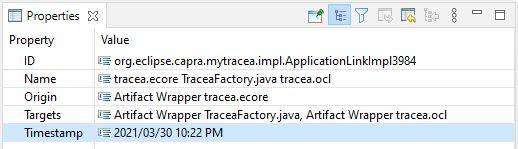
\includegraphics[width=.65\linewidth]{images/properties.jpg}
	\caption{Links are viewed and edited with Eclipse Properties view}
	\label{fig:properties}
\end{figure}
Traces are serialized into an Ecore model, stored in an XMI file. Artefacts wrappers are also stored in XMI.
The \texttt{Reflexive Ecore Model Editor} (together with the \texttt{Properties} view, see  \Fig{fig:properties}) can be used to edit the information but \textbf{the consistency of other views is not guarantied.} Eclipse must be closed and reopened.
The name of the files appear in the project list, but their name cannot be edited. 
\textbf{It is highly recommended to not modify the files, nor delete them.} The default \texttt{PlantUML viewer} does not offers any means to interact with the trace.


\subsection{Trace quality evaluation}
Capra checks the consistency of traces when artefacts are modified or deleted through the Eclipse platform. Changes in the software elements triggers a validity check on the links these elements take part in (as source or target). As a consequence, the links are tagged with a warning. There is no fix proposed.

Confidence is not quantified and there is no record of the facts or evidences about the existence of a link.

\subsection{Conclusion}

Table \ref{tab:evaluationcapra} summarizes the evaluation of Capra, and \Fig{fig:evaluationcapra} illustrates the summary with regard to the traceability infrastructure overview. As can be seen, the tool benefits a strong customization potential. On the one hand, it is easy to design wrappers for new artefacts with Eclipse \texttt{IResource} redefinition, and the definition of link types is very expressive thanks to XCore.   
On the other hand, if the tool lacks some automated mechanisms to identify traces, the visualization of both specific links and derived UML relations is very powerful. 
Capra is currently used in three use cases: Change Impact Analysis, Coverage analysis, and Safety analysis, with a publication to come on these matters. 

On a bad note, the absence of means to edit safely trace links is a major impediment to the use of Capra in an industrial context. Discussing with the authors on the matter showed there is no plan to address this issue. They do not consider the use of the XMI editor as a convenient mean to edit traces.

The tool also suffers a lack of trace quality assessment. 
There is one feature related to quality in Capra which consists in a consistency check that triggers warnings when resources targeted by traces are modified or deleted in the Eclipse environment.
Yet, there is no evaluation of any kind of confidence level and less explainability resources. This is a recurrent limitations that most if not all traceability solutions suffer~\cite{batot2020-survey-driven-feature-model,batot2021-not-another-metamodel}. 


As a conclusion, Capra is a rather good tool for traceability in terms of adaptativeness -- and that is a very important concern to tracer design. The quality of trace links is not considered, as expected -- but we show in the next section how to extend Capra with Trace\textit{a} to circumcise this limitation.

\begin{table}[h]   
	\centering
	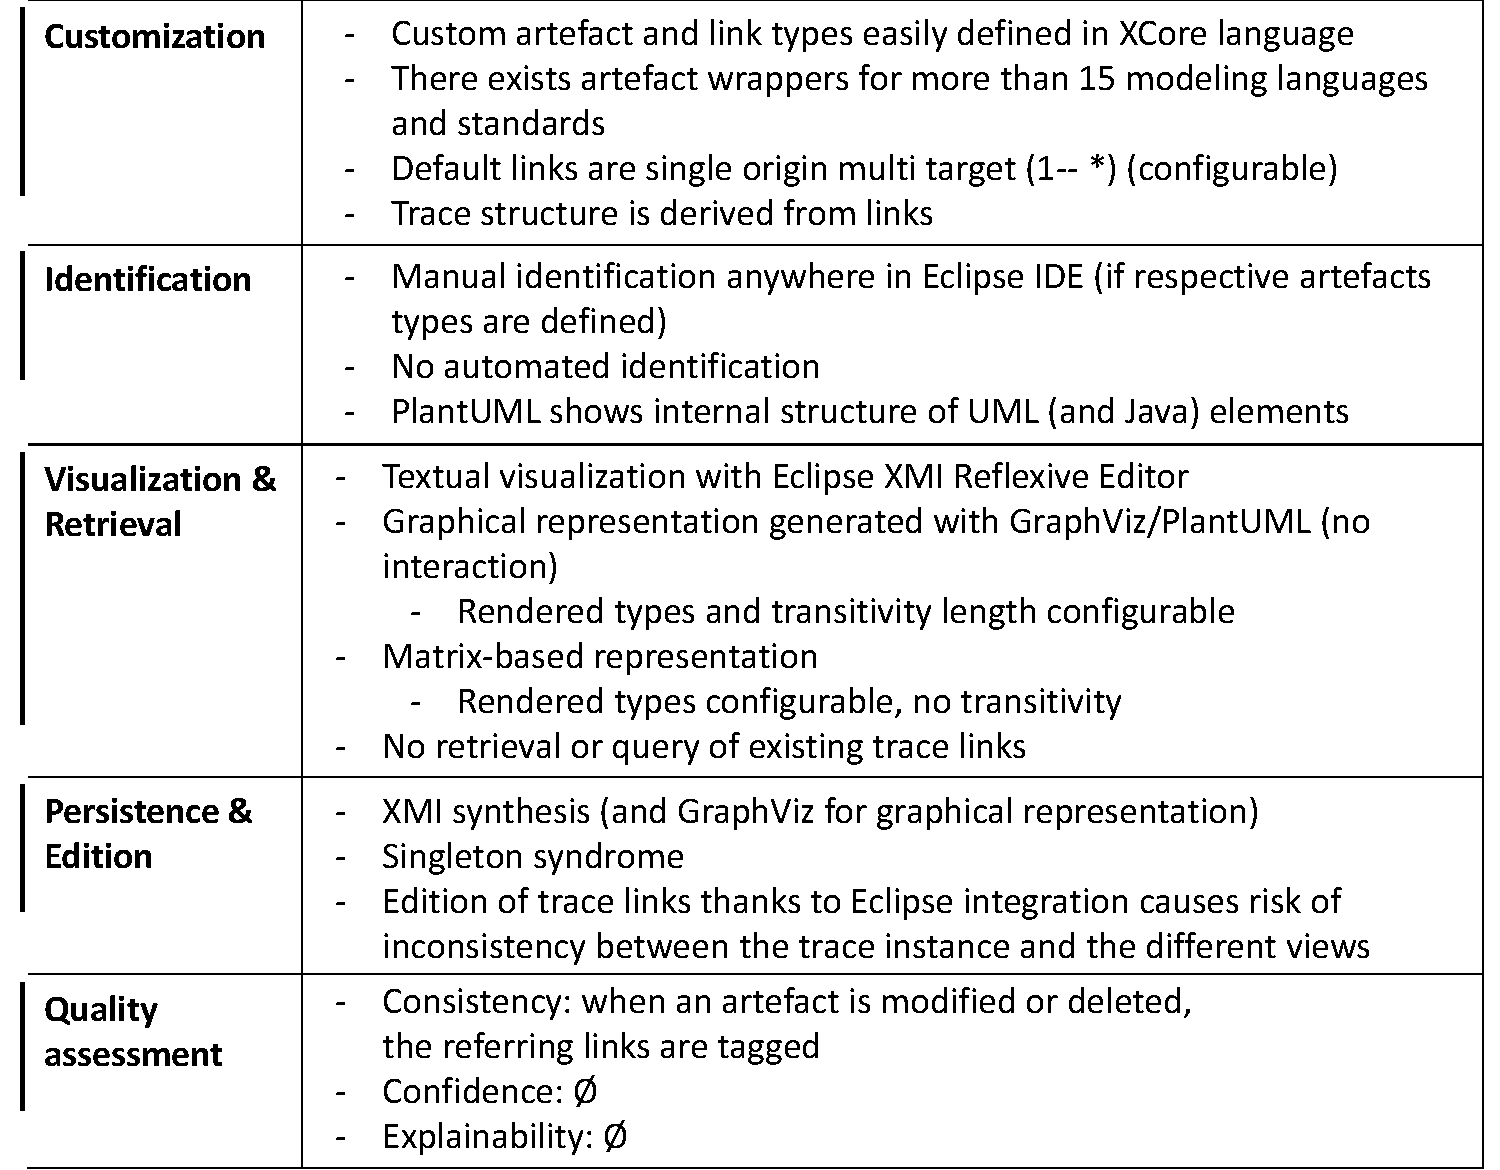
\includegraphics[width=.85\linewidth]{images/evaluation-table-capra.pdf}
	\caption{Summary of the evaluation of Capra}
	\label{tab:evaluationcapra}
\end{table}
\begin{figure}[h]  
	\centering
	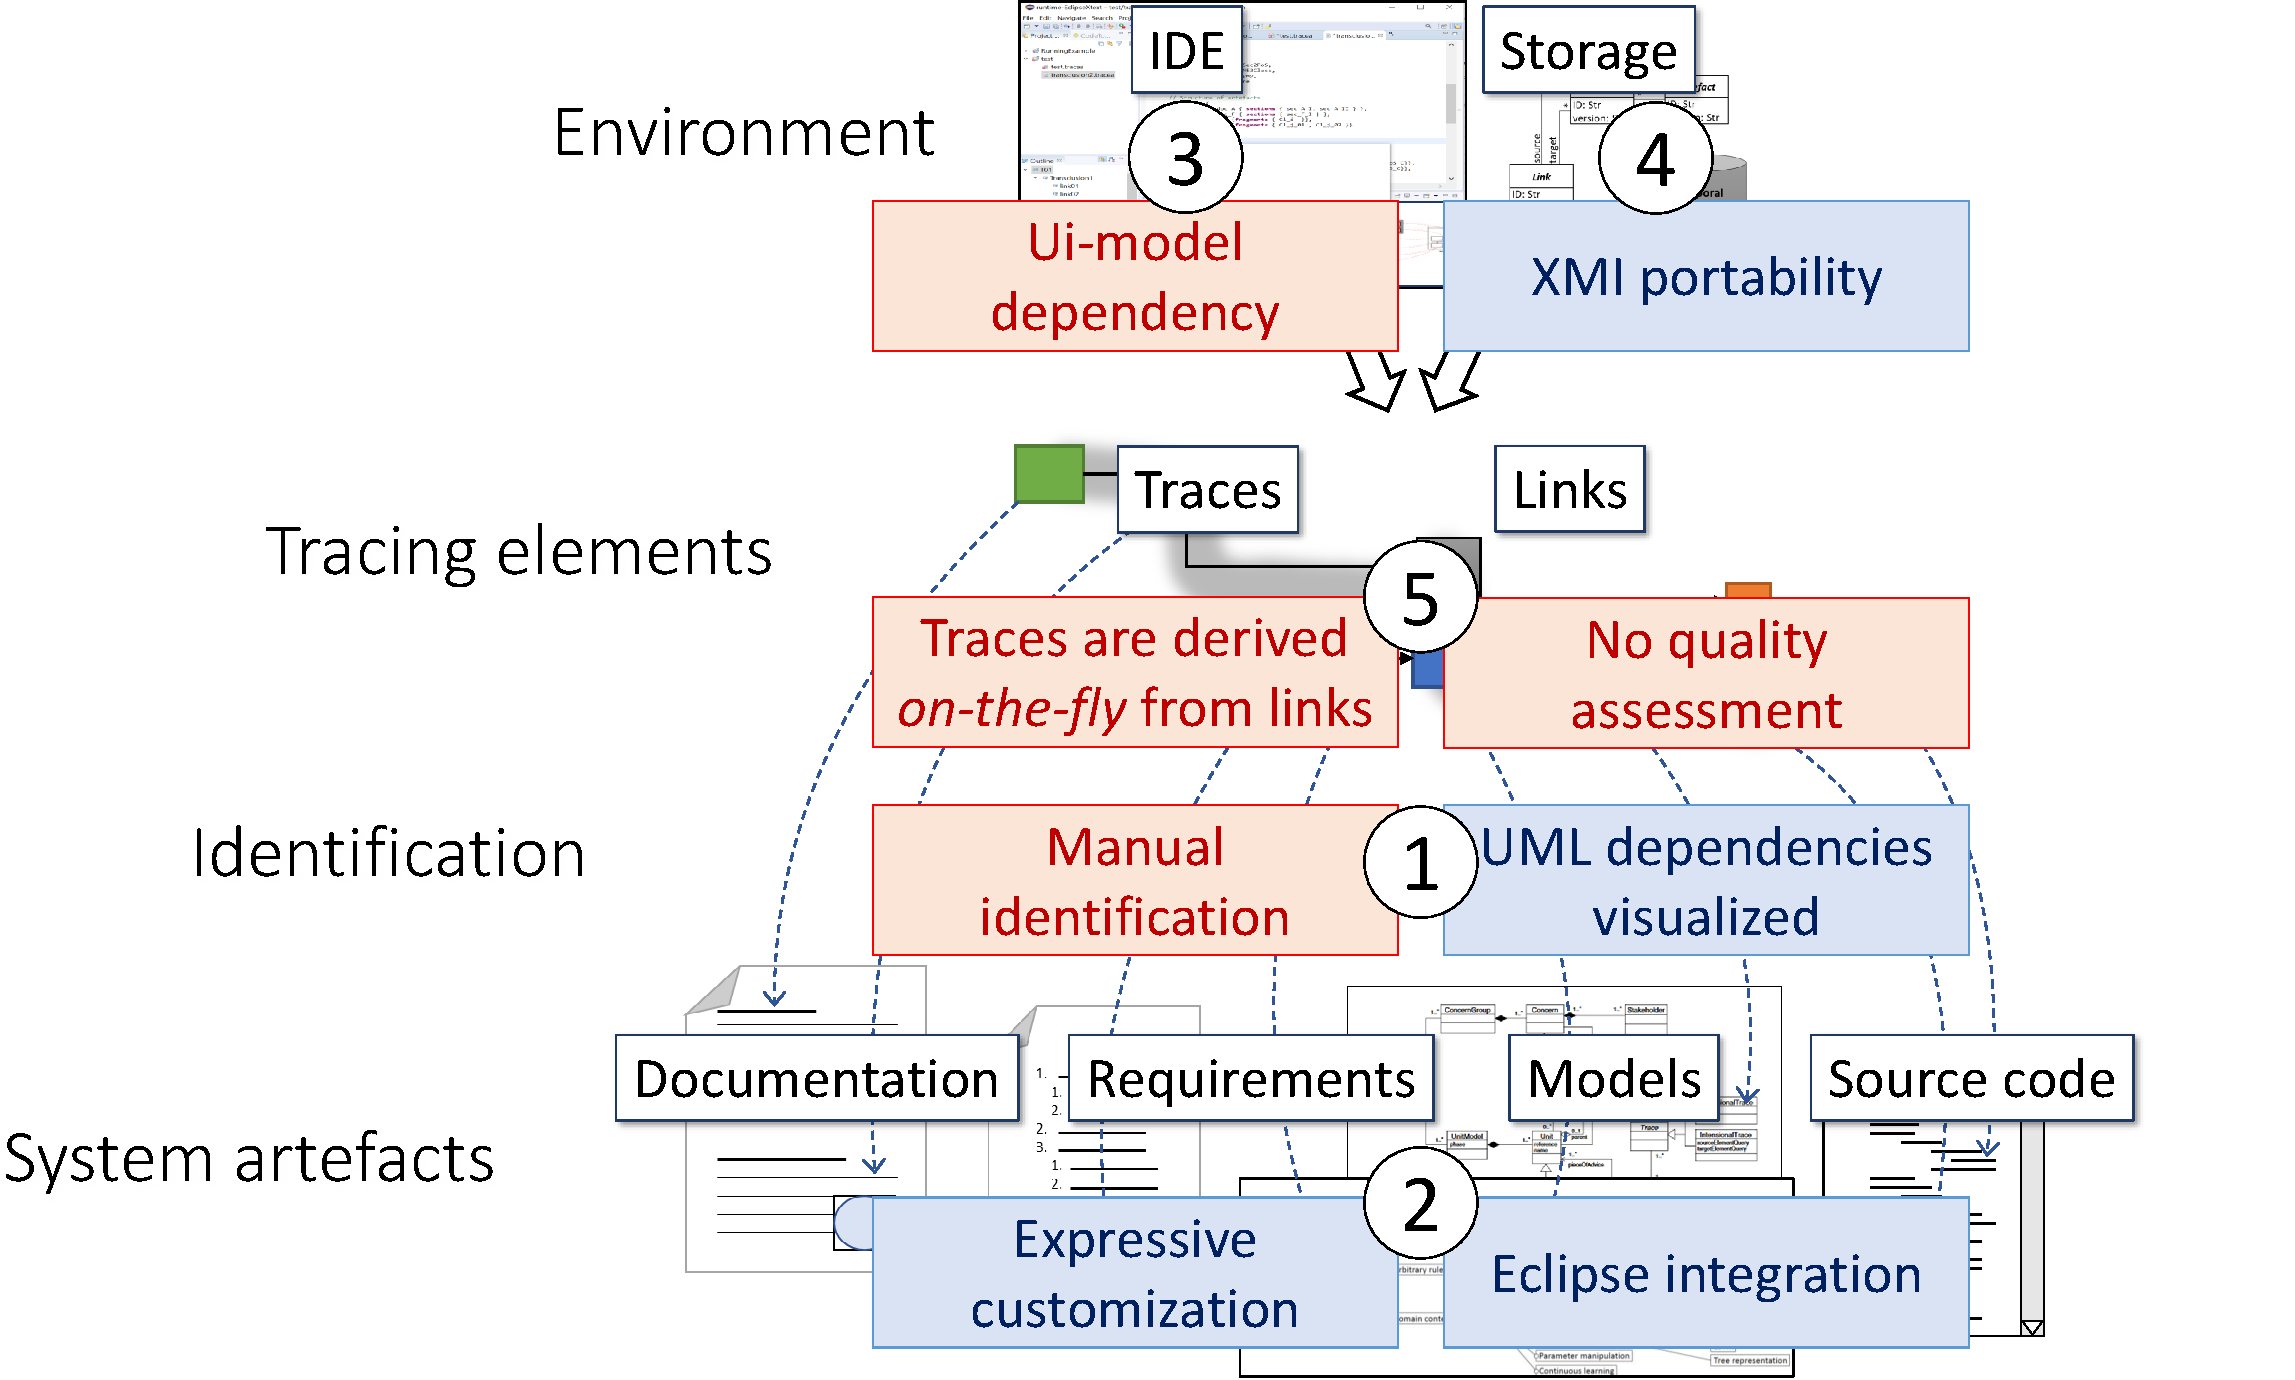
\includegraphics[width=.7\linewidth]{images/evaluation-points-capra.pdf}
	\caption{Summary of the evaluation of Capra}
	\label{fig:evaluationcapra}
\end{figure}


\section{Metadata feature library for quality traceability}\label{sec:extension}

\sideboxbegin{o}
This section presents the limitations imposed by the state of the art of KerML / SysMLv2 in terms of meta-annotation. It then presents the design that we have implemented to overcome it.
\sideboxend
We have previously mentioned the advantages that the use of feature libraries  (orthogonal) offers compared to more intrusive strategies (modifying the structure of the language).

However, the development of datatypes dedicated to traceability encounters a certain number of limitations due to the state of progress of the implementation of KerML / SysMLv2. In this section, we present the limitations encountered and then our design for quality traceability for KerML \textit{and} SysMLv2.

\subsection{Orthogonality - priority and limitations}\label{sec:orthogonalite}
 
\begin{figure}[ht]     
	\centering
	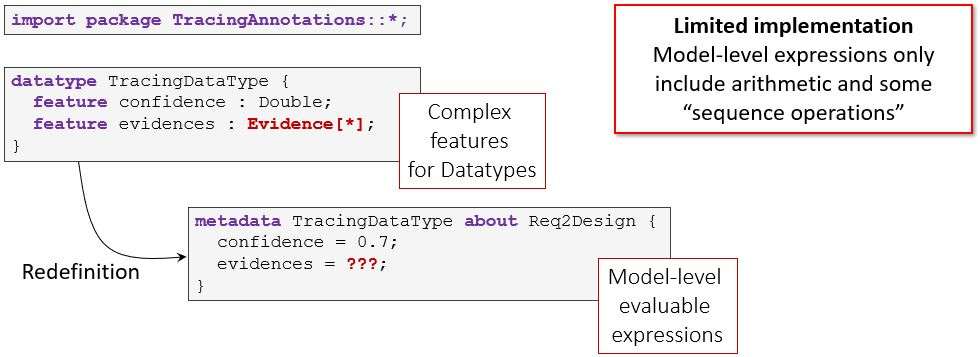
\includegraphics[width=.99\linewidth]{images/strategy4-metadatatype.jpg}
	\caption{Defining complex Metadata structures and evaluating expressions at model level: implementation limits. }
	\label{fig:strategy4}
\end{figure}


To use the words of Ed Seidewitz, one of the main promoters of the new version of SysML and one of the main people responsible for its delivery, the idea of using the AnnotatingFeatures to define \textit{a priori} external needs to the language specifications is "extremely relevant". However, the next revision will not contain any specific article on the matter. A number of decisions remain to be clarified on the subject.
In particular, the ability to define and reuse complex structures within feature datatypes is under consideration. For now, the definition of complex datatype is not guaranteed to work, as illustrated in \Fig{fig:strategy4}.

\begin{figure}[ht]     
	\centering
	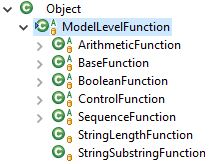
\includegraphics[width=.35\linewidth]{images/modellevelfunction-type-hierarchy.JPG}
	\caption{Types of functions available for evaluating expressions at the model level.}
	\label{fig:modellevelfunc}
\end{figure}

Until the delivery of the second revision (RFP2) scheduled for late August 2021, the SST remains busy with other priorities. Ed Seidewitz foresees the deployment of the features related to modelv level expression in October or November 2021. At the time of writing, annotating features are "only" templates in which some points of variability are allowed (the authorized functions are derived from ModelLevelFunction, see \Fig{fig:modellevelfunc}).

Consequently, the definition of complex structures within datatypes is limited as stated above. Only Ed Seidewitz is aware of the code related to the question and he himself struggles to remember the state of the module dedicated to the assignment of values to complex datatypes. As an example, the use of enumeration (\textit{enum}) in annotations does not allow their use for evaluation (see \Sect{sec:filter}). 
Finalizing this implementation will only be possible when a subset of the modeling language SysML will be defined. In view of the SST's plans to converge the different types of annotations towards AnnotatingFeatures using metadatatypes, these points will be addressed with high priority -- but only after the submission of the new revision.

\subsection{Iterative design: confidence and explainability of trace links}\label{sec:design}
\begin{figure}[ht]      
	\centering
	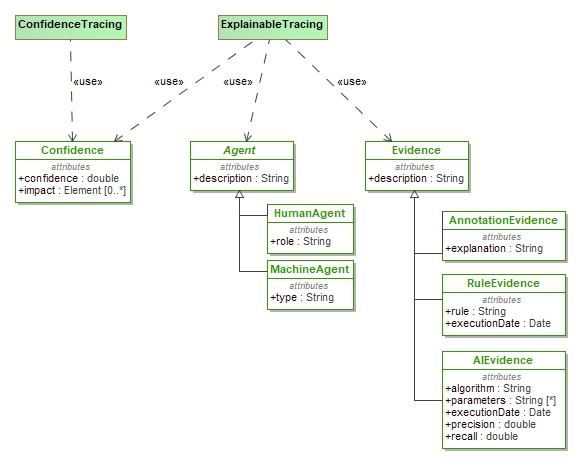
\includegraphics[width=.9\linewidth]{images/explainability-datatype.jpg}
	\caption{Metadatatypes for quality traceability including an assessment of confidence and monitoring of the identification processes used.}
	\label{fig:datatypes}
\end{figure}

To favor the use of specialized libraries (such as the SST encourages), we have designed SysML and KerML datatypes dedicated to tracing. 
\Fig{fig:datatypes} shows the design of these structures. At the top, we distinguish between a design allowing the assessment of confidence and a design allowing to go further by entering the supporting information for this assessment.
We distinguish between the two for the sake of iterativity of the development and implementation processes (as we have just seen, the mechanisms allowing the manipulation and evaluation of datatypes are not fully completed in KerML / SysMLv2).

The \texttt{ConfidenceTracing} datatype has been implemented to overcome this disappointment and initially allows the attribution of a real value of confidence to the annotated links. We add a description field (free String) and a field to reference to potentially impacted elements -- \textit{e.g.,} used in the calculation of the confidence value.
The \texttt{ExplainableTracing} datatype has the same attributes as ConfidenceTracing (description, confidence and impact) with in addition \textit{i)} the notion of Evidence to store information about the identification process used for tracing, and \textit{ii)} the possibility to inform which (type of) agent is responsible for identification.

\subsection{Consequence of the separation of KerML and SysML languages}\label{sec:lggsep}
SysML is based on KerML. However, if the language dedicated to systems reuses the concepts of the kernel language, these are not accessible from the former. Thus, the definition of a Datatype (and its associated Features) does not work in SysML but only in KerML. To allow the use of Trace\textit{a} in both languages, we have transformed the Datatypes and their features into \textit{attribute definitions and uses} (resp. "Attribute def" and "Attribute"). Indeed, an attribute definition is a particular type of structure dedicated to the construction of Datatypes for the design of systems (see \Fig{fig:dtnattributes}).


\begin{figure}[h]     
	\centering
	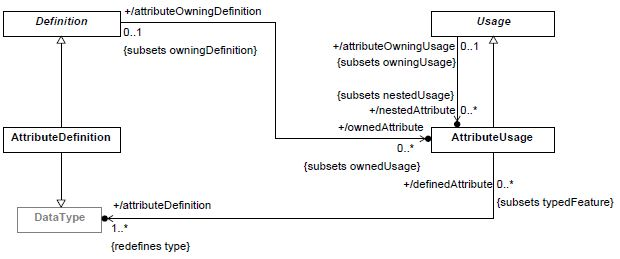
\includegraphics[width=.9\linewidth]{images/dtnattributes.JPG}
	\caption{The definition and use of attributes in SysML is a specialization of datatypes and their features in KerML.}
	\label{fig:dtnattributes}
\end{figure} 

\subsection{Usage example: filtering}\label{sec:filter}
This section presents an example: the filtering of links satisfying a confidence greater than a given threshold.
The first 30 lines of listing~\ref{lst:filter} (with graphical representation in \Fig{fig:vizfilter}), show the structure of the system and links being traced. Lines 33 to 39 show the code needed for filtering. This is a reuse of the existing machinery to support SysMLv2 metadata annotations. \Fig{fig:vizfilterres} shows the result of the query: the five links with a confidence greater than 0.5 are filtered.

% \pagebreak
\begin{lstlisting}[caption={Definition and filtering of tracing annotations to collect links satisfying a certain level of confidence.},
label=lst:filter,
style=mystylesysml,
linewidth=16cm,
xleftmargin=1.7cm,
morekeywords={part,filter}]
package Tracing_FilterExample {
	import TracingAnnotations::*;
	
	/* System under tracing. */
	part end1 {}
	part end2 {}
	part end3 {}
	part end4 {}
	part end5 {}
	part end6 {}
	part end7 {}
	part end8 {}
	
	/* Trace links, confidence valued. */
	connection testLink95 connect end1 to end2 
	  {@ConfidenceTracing { confidence = 0.95; }}
	connection testLink85 connect end1 to end3 
	  {@ConfidenceTracing { confidence = 0.85; }}
	connection testLink75 connect end1 to end4 
	  {@ConfidenceTracing { confidence = 0.75; }}
	connection testLink65 connect end5 to end6 
	  {@ConfidenceTracing { confidence = 0.65; }}
	connection testLink55 connect end6 to end7 
	  {@ConfidenceTracing { confidence = 0.55; }}
	connection testLink45 connect end7 to end8 
	  {@ConfidenceTracing { confidence = 0.45; }}
	connection testLink35 connect end8 to end7 
	  {@ConfidenceTracing { confidence = 0.35; }}
	connection testLink25 connect end8 to end6 
	  {@ConfidenceTracing { confidence = 0.25; }}
}

import TracingAnnotations::*;
/* Filter example - full notation. */
package ConfidenceLevel {
	/*Connections that satisfy a threshold confidence level (0.5).*/
    import Tracing_FilterExample::**;
    filter @ConfidenceTracing && ConfidenceTracing::confidence >= 0.5;
}
\end{lstlisting}


\begin{figure}[ht]     
	\centering
	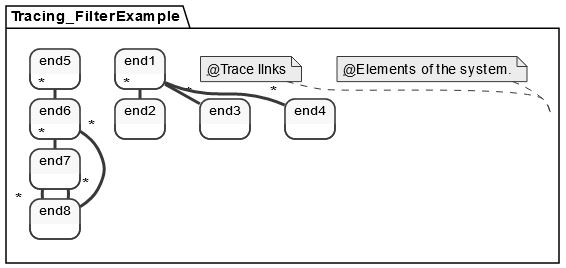
\includegraphics[width=.9\linewidth]{images/viz_filterexample.JPG}
	\caption{Example using the SysMLv2 filtering tool for trace annotations.}
	\label{fig:vizfilter}
\end{figure} 

\begin{figure}[ht]     
	\centering
	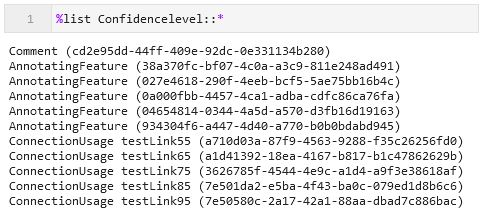
\includegraphics[width=.75\linewidth]{images/viz_filterexample_res.JPG}
	\caption{Filtering result: filtered annotations (\textit{i.e.,} satisfying a specific confidence).}
	\label{fig:vizfilterres}
\end{figure} 



The same process can (could) be used to "tag" links with specific types -- or any other pre-defined attribute. The implementation of the evaluation of expressions is unfortunately limited. As to this day, the use of strings of characters (\textit{String}) or of enumerations (\textit{enum}) in the definition of datatypes generates a compilation error. \Fig{fig:vizfiltererr} shows this limitation (the figure has been generated with JupyterLab, see \Sect{sec:artefacts}).

\begin{figure}[ht]     
	\centering
	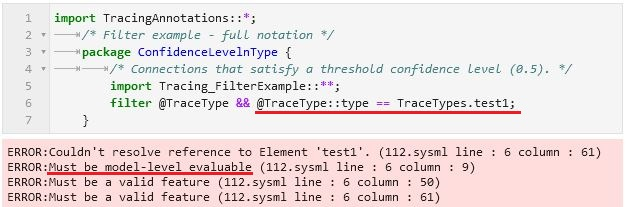
\includegraphics[width=.9\linewidth]{images/viz_filterexample_err.JPG}
	\caption{Filtering is not (yet) implemented for enumerations.}
	\label{fig:vizfiltererr}
\end{figure} 

\section{Limitations of the Capra solution}\label{sec:limitations}

\sideboxbegin{o}
This section shows Capra's limitations in term of software design. The singleton syndrome and the absence of link editor being the most salient limitations to plan an industrial exploitation of the tool.
\sideboxend

The ability of Capra to represent traces and customize relationships and artefacts is promising. Nonetheless, the tool implementation suffers important limitations. In this section, we present architecture flaws that would restrain an industrial exploitation of Capra.  We show the technical limitations at design and code level that need to be addressed.

\subsection{Singleton syndrome}
The main limitation of Capra lies in the design choices made to implement traces. Its architecture implies that using Capra remains only a one shot deal. There is one file to store links. "Traces", or better said \textit{the trace}, is regenerated from this file at startup. If the user wants to create different \textit{traces}, s.he will have to start a new instance of Capra with a new XMI file.
This is what we call the \textit{singleton syndrome} where a software (OO) is designed around a unique (often static) instance of its main concept. Capra follows this pattern.

To address this limitation would require a general lift of the manipulation and exploration of traces and links. It would also require modifying high-level architecture of the tool. A report explaining the limitation has been sent to the shareholders of Capra. This issue is under current inspection by the development team. 

\subsection{Single step trace links}
The next limitation is that Capra does not offer any opportunity to synthesized the trace structure. The trace is derived from the trace links on demand for visualization only. 
The way a trace is derived can be configured freely in the trace model implementation (see \verb|org.eclipse.capra.TraceMetaModelAdapter|) but can only describe one trace due to the previous limitation.

A solution could be buffering derived traces to avoid reconstructing them to often. Otherwise, without optimization, the tool will hardly scale.

\subsection{Trace edition shortfall}
We use the XMI Reflexive Model Editor to edit trace links and attribute them confidence value and properties. This shall be improved in the future because for now, there is no assertion that the over views on the trace instance remain consistent between one another. In other wother words, modifying trace links through this editor implies to restart Eclipse to take these changing in consideration. 

The development team is aware of this limitation but does not plan to address it, considering that the edition of trace links is of no use.

\subsection{Naming convention and general quality}
The use of a \texttt{Connection} adapter for links is sometimes misleading. In the PlantUML viewer, the trace links show their corresponding origins and targets whereas EMF elements show their internal structure. The later is defined in the wrappers of the artefact model as described in Section \ref{sec:evaluationcapra}.  

"Trace", "Link", "Connection", "Connections", "TraceLink" sometimes collide in method and attribute signatures.  \textit{E.g.}, In \verb|AbstractTraceMetamodel.createTrace| and  \verb|AbstractTrace-| \verb|Metamodel.deleteTrace| "trace" entities are actually connections. Which is fundamentally misleading.

There can be found cut-n-pastes as well which we should be careful about, specifically in the generic trace model (\verb|org.eclipse.capra.generic.tracemodel|), and the generation of PlantUML diagrams (in \verb|org.eclipse.capra.ui.plantuml.DiagramTextProviderHandler|).


% \subsection{Singleton syndrome} 
% \subsection{Architecture flaws}
% \begin{descriptioncompact}
% \item[Single step trace links] 

% \item[Concerns overlap] 


% \item[Naming convention and general quality] 


% \end{descriptioncompact}



\section{Conclusion}\label{sec:conclusion}
% \begin{descriptioncompact}
%     \item[Protocol] We propose a protocol to evaluate traceability solution
%     \item[Application] We show an application on Capra.
%     \item[Extension] We detail the extension of Capra as an example of Tracea integration.
%     \item[Limitations] We show Capra's design limitations
% \end{descriptioncompact}

This deliverable presents means to integrate quality traceability into SysMLv2 using Trace\textit{a}.
With Trace\textit{a} datatypes, SysMLv2 relationships can be annotated with valuable information related to their quality -- \textit{i.e.,} their \textit{trustability}. 
The degree of confidence as well as the information necessary to justify it can be associated to SysML links (connections) through metadata definition.


This integration is \textit{orthogonal}. It does not impact the structure of the language itself -- changes happen at the model level with new feature libraries, not at the metamodel level.
This allows the (re)use of the machinery supporting (meta)annotations and eases the (re)definition of tracing structures specific to a certain project or company. We showcase these benefits in one small example that also reveals the current limitations of SysMLv2's implementation.

The SST confirms that annotating features are valuable and salient artefacts in the development of SysML. They shall take more and more importance in the future releases. Work on the evaluation of expressions at the model level is highly required and will be part of the agenda of the fourth quarter of 2021. 
Finally, as a sign of encouragement, the SST invites us to further investigate in the direction we took. 

\section{Software artefacts}\label{sec:artefacts}
The software artifacts we have implemented have been uploaded to the Modelia Git repository and can be accessed at:
\url{https://github.com/modelia/tracea/3-sysml-integration}.

The file contains the two definitions presented above along with a simple example and a filtering usage example. Subfolders are \verb|/kerml| and \verb|/sysml| respectively to KerML and SysML versions.

SysML datatypes can be viewed in the JupyterLab of the SST. To do so, open the following link (\url{https://www.sysmlv2lab.com/}) in a web browser  and upload the code contained in \verb|/sysml/jupyterlab/TraceaTracingAnnotations.ipynb| from the Tracea Git repository. Its Markdown counterpart ($.md$) shows a \textit{Git readable} version of the Jupyter document.


%\appendix

%\cleardoublepage

%\section{Appendix}
%\includepdf[pages=-]{paper/MODELS_19_Submission.pdf}
%\label{sec:AppendixPaper}

%\input{sections/aa-appendix}

% Bibliography
%%%%%%%%%%%%%%%%%%%%%%%%%%%%%%%%%%%%%%%%%%%%%%%%%%%%%%%%%%%%%%%%%%%%%%

\cleardoublepage
\bibliographystyle{plain}
\bibliography{bib/strings-abbr,bib/trace-and-models,bib/uoc2020_tracea,bib/added}

% Clarifications
%%%%%%%%%%%%%%%%%%%%%%%%%%%%%%%%%%%%%%%%%%%%%%%%%%%%%%%%%%%%%%%%%%%%%%

% Print them only if the notes package is loaded (c@pagenode exists)
% and there are notes defined within the document (pnotesavechap > 0)

\makeatletter
\ifcsname c@pagenote\endcsname
\ifthenelse{\value{pnotesavechap}>0}{\cleardoublepage\printnotes}{}
\fi
\makeatother

%\makeback

\end{document}          
